\renewcommand{\thispart}{3}
\renewcommand{\thispartname}{
  Introduction to Deep Networks and\\
  Automatic Differentiation (Backpropagation)
}

\part{\thispartname}

% Cover page
%
% Cover page for giveb part
%

\title[\modulename - Part \thispart]
{
  {\bf 
   \modulename - 
   Part \thispart\\
  }
  \vspace{0.5cm}
  {\it 
   \color{yellow}
    \secname\\
  }
}
\author[C.Andreopoulos] {
  Professor Costas Andreopoulos\inst{1,2}, {\it FHEA}
}
\institute[Liverpool/STFC-RAL] {
   \inst{1} University of Liverpool, Department of Physics\\
   \vspace{0.3cm}
   {\it {\color{magenta} Lectures delivered at the University of Liverpool, 2024-25}}\\
   \vspace{0.2cm}
}
\date{\today}

\titlegraphic{
  
\includegraphics[height=30px]{images/logo/liverpool.png}
}

\begin{frame}[plain]
  \titlepage
\end{frame}




% Outline
\section{Outline}
%
% Table of contents to be displayed at the beginning of each part
%

\begin{frame}[t,allowframebreaks]{Outline for Part \thispart -}
  % Part \thispart (\secname) covers the following topics:\\
  % \vspace{0.5cm}
  \linespread{1.1}
  \setcounter{secnumdepth}{3}
  \setcounter{tocdepth}{3}
  % \tableofcontents[currentsection, hideothersubsections, sectionstyle=hide/hide]
  \tableofcontents[part=\thispart]
\end{frame}



% Learning XOR
% Illustrate limitations of linear model and the
% power of nonlinear models to learn new representations
\section{Learning the XOR function}
%
% Learning the XOR function
%

\begin{frame}[t,allowframebreaks]{Learning the XOR function -} 

    The XOR (exclusive or, or exclusive disjunction) function
    is an operation on two variables that take binary values (0,1).\\
    \vspace{0.2cm}

    \begin{columns}[t]
        \begin{column}{0.32\textwidth}
            \vspace{-1.1cm}
            \begin{center}
                \begin{tabular}{ c c | c }
                 $x_1$ & $x_2$ & $y = x_1 \oplus x_2$ \\ 
                 \hline
                 0 & 0 & 0 \\  
                 0 & 1 & 1 \\   
                 1 & 0 & 1 \\  
                 1 & 1 & 0 \\   
                \end{tabular}
                %\label{tab:xor_truth}
            \end{center}
        \end{column}
        \begin{column}{0.68\textwidth}
            Let $x_1$, $x_2$ be the two input binary values
            and $y$ be the output of the operation, denoted as $x_1 \oplus x_2$.\\
            \vspace{0.2cm}
            $y$ is 1 only if exactly one of $x_1$, $x_2$ is 1.\\ 
            \vspace{0.2cm}
            The full truth table is given on the left.\\
        \end{column}
    \end{columns}

    \vspace{0.3cm}

    We would like to construct a model 
    $f(\mathbf{x};\mathbf{\theta}):\{0,1\}^2\rightarrow\{0,1\}$ 
    that {\bf learns the XOR function} 
    by adjusting the parameters in $\mathbf{\theta}$.
    \begin{itemize}
        \item 
        This function is defined only for 
        4 points $\mathbf{x}=(x_1,x_2)^T$.
        \begin{itemize}
         \item 
         $\mathbf{x} \in \mathbb{X} 
          = \{(0,0)^T, (0,1)^T, (1,0)^T, (1,1)^T\}$.
        \end{itemize}
        \item 
        The training set $\mathbb{D}$ contains 
        4 training examples $(\mathbf{x},y)$,
        constructed from $\mathbf{x} \in \mathbb{X}$ 
        and the truth table given above.
    \end{itemize}

\framebreak

    We can treat this as a regression problem, and use a 
    \gls{mean square error loss function}:
    \begin{equation}
        \mathcal{L}(\mathbf{\theta}) =  
        \frac{1}{4} 
        \sum_{(\mathbf{x},y) \in \mathbb{D}} 
        (y - f(\mathbf{x};\mathbf{\theta}))^2
        \label{eq:learn_xor_loss_function_1}
    \end{equation}
    This is not an ideal choice for binary data,
    but it is a simple choice which is sufficient for our purposes.\\
    \vspace{0.2cm}

    What remains, is to specify the form of the model 
    $f(\mathbf{x};\mathbf{\theta})$.

\end{frame}

\subsection{Applying a linear model to the XOR regression task}
%
%
%

\begin{frame}[t,allowframebreaks]{
    Applying a linear model to the XOR regression task -} 

    We can choose a linear form for the model $f(\mathbf{x};\mathbf{\theta})$,
    where the parameter set $\mathbf{\theta}$ consists 
    of a set of weights $\mathbf{w}$ = $(w_1,w_2)$ and a bias $b$.        

    \begin{columns}[t]
        \begin{column}{0.50\textwidth}
            \vspace{-0.6cm}
            \begin{center}
                \begin{tikzpicture}[scale=1]
                  %\draw[help lines] (0,0) grid (6,3.7);
                  \node[ann_processing_node] (o)  at (3.0, 1.5) {$\sum$};
                  \node[ann_input_node]      (x1) at (0.0, 3.0) {$x_1$};
                  \node[ann_input_node]      (x2) at (0.0, 1.5) {$x_2$};
                  \node[ann_bias_node]       (b)  at (1.0, 0.0) {$+1$};
              
                  \drawgraphlinebigarrow (x1.east) 
                  to node[above, midway] 
                  {\small $w_1$}(o.north west) ;
              
                  \drawgraphlinebigarrow (x2.east) 
                  to node[above, midway] 
                  {\small $w_2$}(o.west) ;
              
                  \drawgraphlinebigarrow (b.east) 
                  to node[above, midway] 
                  {\small $b$}(o.south west) ;
              
                  \drawgraphlinebigarrow (o.east) 
                  to node[above,midway] 
                  {\small \color{black} $f(\mathbf{x};\mathbf{w},b)$} (6.0,1.5);              
                \end{tikzpicture}
            \end{center}        
        \end{column}
        \begin{column}{0.50\textwidth}
            \begin{equation}
                f(\mathbf{x};\mathbf{w},b) = \mathbf{x}^{T} \mathbf{w} + b
                \label{eq:learn_xor_linear_model_1}
            \end{equation}

            As discussed previously, we can rewrite 
            Eq.~\label{eq:learn_xor_linear_model_1}
            in a more compact form by adding an additional 
            input $x_0$ that always takes the value of +1 
            and considering the bias $b$ to be the weight $w_0$
            \begin{equation}
                f(\mathbf{x};\mathbf{w}) = \mathbf{x}^{T} \mathbf{w}
                \label{eq:learn_xor_linear_model_2}
            \end{equation}
        \end{column}
    \end{columns}
      
    \framebreak

    %
    %

    The \index{loss function}\gls{loss function} 
    of Eq.~\ref{eq:learn_xor_loss_function_1} 
    could be minimised using the 
    \index{gradient descent}\gls{gradient descent} 
    method which was briefly mentioned before 
    (and will be studied further in following lectures).\\
    \vspace{0.1cm}
    Owing to the simplicity of the given 
    \index{regression}\index{linear regression}\gls{regression} problem, 
    it is possible to obtain a solution in closed form 
    (see derivation of 
    Eq.~\ref{eq:linear_regression_closed_form_solution_matrix}).\\
    \vspace{-0.2cm}
    \begin{equation*}
        \vect{w} = (\vect{X}^T \vect{X})^{-1} \vect{X}^T \vect{y}
    \end{equation*}\\
    \vspace{0.1cm}
    The training set $\mathbb{D}$ contains 4 examples 
    $(\mathbf{x}^{(i)},y^{(i)})$, with $i \in [1,4]$, given in the table below.\\
    \vspace{0.1cm}
    \begin{columns}[t]
        \begin{column}{0.44\textwidth}
            \vspace{-0.6cm}
            \begin{center}
                \begin{tabular}{ c | c c c | c }
                 $i$ & $x_0$ & $x_1$ & $x_2$ & $y = x_1 \oplus x_2$ \\ 
                 \hline
                 1 & 1 & 0 & 0 & 0 \\  
                 2 & 1 & 0 & 1 & 1 \\   
                 3 & 1 & 1 & 0 & 1 \\  
                 4 & 1 & 1 & 1 & 0 \\   
                \end{tabular}
            \end{center}
        \end{column}
        \begin{column}{0.56\textwidth}
            The inputs $\mathbf{x}^{(i)}$ and target values
            $y^{(i)}$ spanning $\mathbb{D}$ can be packed into matrices
            as shown in Eq.~\ref{eq:linear_regression_closed_form_solution_matrix_inputs}.
            \begin{equation}
                \vect{X} = 
                \begin{pmatrix}
                    1 & 0 & 0 \\
                    1 & 0 & 1 \\
                    1 & 1 & 0 \\
                    1 & 1 & 1 \\
                \end{pmatrix} 
                \; \textrm{and} \;
                \vect{y} = 
                \begin{pmatrix}
                    0 \\
                    1 \\
                    1 \\
                    0 \\
                \end{pmatrix} 
            \end{equation}        
        \end{column}
    \end{columns}

    \framebreak

    %
    %

    The matrix product $\vect{X}^T \vect{X}$ is:\\
    \vspace{-0.3cm}
    \begin{equation}
        \vect{X}^T \vect{X} = 
        \begin{pmatrix}
            1 & 1 & 1 & 1 \\
            0 & 0 & 1 & 1 \\
            0 & 1 & 0 & 1 \\
        \end{pmatrix} 
        \begin{pmatrix}
            1 & 0 & 0 \\
            1 & 0 & 1 \\
            1 & 1 & 0 \\
            1 & 1 & 1 \\
        \end{pmatrix} =
        \begin{pmatrix}
            4 & 2 & 3 \\
            2 & 2 & 2 \\
            2 & 1 & 2 \\
        \end{pmatrix} 
    \end{equation}        

    while its inverse, as it can be easily verified, is:\\
    \vspace{-0.3cm}
    \begin{equation}
        (\vect{X}^T \vect{X})^{-1} = 
        \begin{pmatrix}
            0 & -0.5 & -1 \\
            0 &  1   & -1 \\
           -1 &  0   &  2 \\
        \end{pmatrix} 
    \end{equation}        
    \vspace{-0.5cm}
    Substituting the above matrices 
    in Eq.~\ref{eq:linear_regression_closed_form_solution_matrix}, we find:\\
    \begin{equation}
        \vect{w} 
        = 
        \begin{pmatrix}
            b   \\
            w_1 \\
            w_2 \\
        \end{pmatrix} 
        =
        \begin{pmatrix}
            0 & -0.5 & -1 \\
            0 &  1   & -1 \\
           -1 &  0   &  2 \\
        \end{pmatrix} 
        \begin{pmatrix}
            1 & 1 & 1 & 1 \\
            0 & 0 & 1 & 1 \\
            0 & 1 & 0 & 1 \\
        \end{pmatrix} 
        \begin{pmatrix}
            0 \\
            1 \\
            1 \\
            0 \\
        \end{pmatrix} 
        =
        \begin{pmatrix}
            0.5 \\
            0 \\
            0 \\
        \end{pmatrix} 
        \label{eq:learn_xor_linear_model_weights}
    \end{equation}        

    \framebreak

    %
    %

    The estimated model parameters $\mathbf{w}^T=(0.5, 0, 0)$,
    substituted in Eq.~\ref{eq:learn_xor_linear_model_2}, 
    yield the following predictions:\\
    \vspace{0.4cm}
    \begin{equation}
        \hat{y}(\mathbf{x}) = 
        \begin{pmatrix}
            1 & x_1 & x_2 \\
        \end{pmatrix} 
        \begin{pmatrix}
            b   \\
            w_1 \\
            w_2 \\
        \end{pmatrix} =
        \begin{pmatrix}
            1 & x_1 & x_2 \\
        \end{pmatrix} 
        \begin{pmatrix}
            0.5 \\
            0   \\
            0   \\
        \end{pmatrix} = 0.5
        \label{eq:learn_xor_linear_model_predictions}
    \end{equation}

    Therefore, irrespective of the input $\mathbf{x}$, the {\bf model always returns 0.5}, 
    halfway between the two possible target values of 0 and 1.\\
    \vspace{0.2cm}
    This is a rather {\bf spectacular failure} for our trained linear model.

\end{frame}

%
%
%

\begin{frame}[t,allowframebreaks]{Linear models cannot learn the XOR function -} 

    \begin{columns}[t]
        \begin{column}{0.50\textwidth}
            \begin{center}
                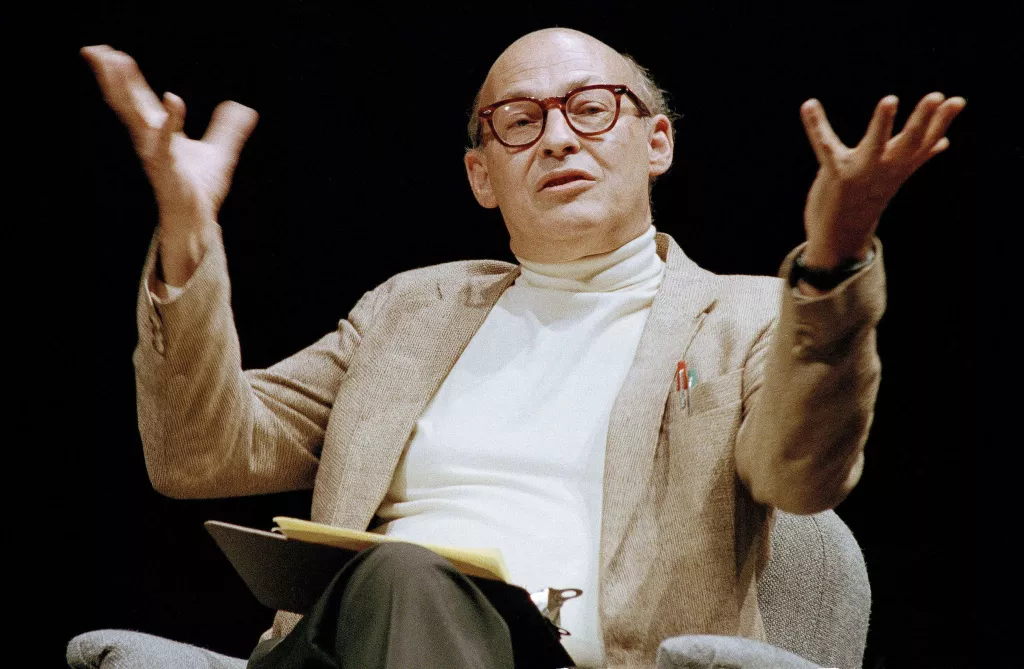
\includegraphics[width=0.90\textwidth]
                    {./images/people/minsky_1.png}\\
                {\scriptsize 
                Marvin Misky. 
                \color{col:attribution} 
                Photograph by Robert Kaiser (Associated Press).\\}        
            \end{center}
        \end{column}
        \begin{column}{0.50\textwidth}
        \end{column}
    \end{columns}


\end{frame}

\subsection{Applying a nonlinear model to the XOR regression task}
%
%
%

\begin{frame}[t,allowframebreaks]{Nonlinear models can learn XOR -} 

    To solve the problem, we can try a {\bf deeper architecture}.
    \begin{itemize}
        \item 
        For example, we can consider a simple feedforward network 
        with a single hidden layer.\\
    \end{itemize}
    \vspace{0.2cm}

    {\bf What types of functions would be computed} at each layer?\\
    \begin{itemize}
    \item
        {\bf Linear functions have desirable properties}.
    \item
        However, they {\bf they cannot all be linear!}    
        \begin{itemize}
            \item 
            If they were, in spite of its greater depth, 
            the network as a whole would remain a linear function of $\mathbf{x}$
            (and linear models cannot learn XOR).
            % \item 
            % We have just seen that linear models cannot learn the XOR function!
        \end{itemize}
    \end{itemize}
    \vspace{0.2cm}

    We can still use a {\bf linear regression model at the output}.\\
    \vspace{0.2cm}

    However, the {\bf linear model would be applied to transformed features} 
    generated by non-linear functions at the hidden layer.\\
    \vspace{0.2cm}

    In essence, we are {\bf aiming to learn a new representation of the inputs}
    that is linearly separable!\\

    \framebreak

    In essence, we are {\bf aiming to learn a new representation of the inputs}
    that is linearly separable!
    {\bf Representation learning} is a central idea in \gls{dl}.\\

    \begin{center}
        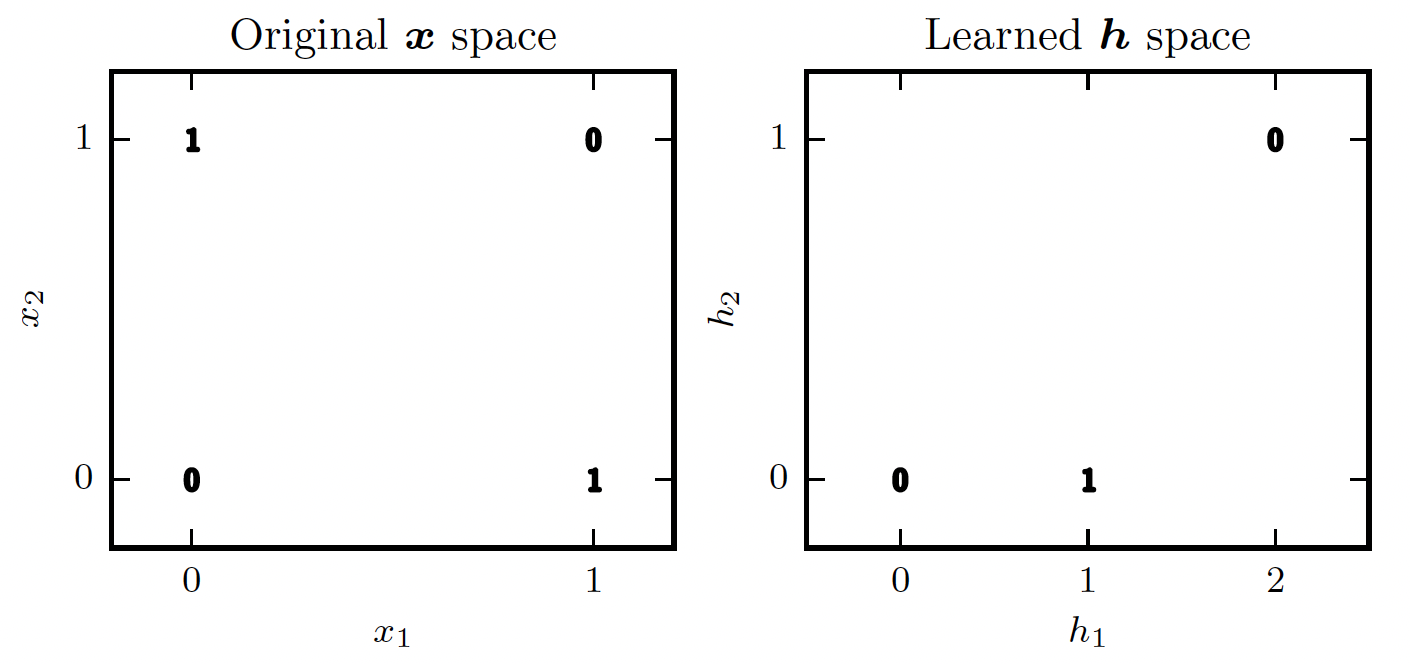
\includegraphics[width=0.90\textwidth]
        {./images/xor/goodfellow17_xor_learned_representations_01.png}\\
     {\scriptsize 
      Solving the XOR problem by learning a representation.\\
      \color{col:attribution} 
      Image reproduced from p. 168 of \cite{Goodfellow:2017MITDL} (Fig. 6.1)}\\
    \end{center}

    \framebreak

    A diagram of our feedforward network is given below.\\
    \begin{center}
        \begin{tikzpicture}[scale=0.98]
          %\draw[help lines] (0,0) grid (8,6);
          \node[ann_processing_node] (o)  at (7.0, 2.5) {$\hat{y}$};
      
          \node[ann_processing_node] (h1) at (4.0, 3.5) {$h_1$};
          \node[ann_processing_node] (h2) at (4.0, 1.5) {$h_2$};
          \node[ann_bias_node]       (b)  at (5.0, 0.0) {$+1$};
      
          \node[ann_input_node]      (x1) at (0.0, 3.5) {$x_1$};
          \node[ann_input_node]      (x2) at (0.0, 1.5) {$x_2$};
          \node[ann_bias_node]       (c1) at (1.0, 5.0) {$+1$};
          \node[ann_bias_node]       (c2) at (1.0, 0.0) {$+1$};
      
          % from input layer to h1
          \drawgraphlinebigarrow (x1.east) 
          to node[above, midway] 
          {\scriptsize $W_{11}$}(h1.west) ;
      
          \drawgraphlinebigarrow (x2.east) 
          to node[below, midway] 
          {\scriptsize $W_{21}$}(h1.south west) ;
      
          \drawgraphlinebigarrow (c1.east) 
          to node[above, midway] 
          {\scriptsize $c_1$}(h1.north west) ;
      
          % from input layer to h2
          \drawgraphlinebigarrow (x1.east) 
          to node[above, midway] 
          {\scriptsize $W_{12}$}(h2.north west) ;
      
          \drawgraphlinebigarrow (x2.east) 
          to node[below, midway] 
          {\scriptsize $W_{22}$}(h2.west) ;
      
          \drawgraphlinebigarrow (c2.east) 
          to node[below, midway] 
          {\scriptsize $c_2$}(h2.south west) ;
      
          % from hidden layer to output
          \drawgraphlinebigarrow (h1.east) 
          to node[above, midway] 
          {\scriptsize $w_1$}(o.north west) ;
      
          \drawgraphlinebigarrow (h2.east) 
          to node[above, midway] 
          {\scriptsize $w_2$}(o.south west) ;
      
          \drawgraphlinebigarrow (b.east) 
          to node[below, midway] 
          {\scriptsize $b$}(o.south) ;
      
          % \drawgraphlinebigarrow (o.east) 
          % to node[above,midway] 
          % {\scriptsize \color{black} $f(\mathbf{h};\mathbf{w},b)$} (10.0,2.5);
      
        \end{tikzpicture}
    \end{center}        

    \framebreak

    The output node computes the function 
    $f^{(1)}: \mathbb{R}^2 \rightarrow \mathbb{R}$
    \begin{equation}
        \hat{y} = 
        f^{(1)}(\mathbf{h};\mathbf{w},b)
        \label{eq:learn_xor_nonlinear_model_f1}
    \end{equation}        
    whereas the hidden layer nodes
    compute the function
    $f^{(2)}: \mathbb{R}^2 \rightarrow \mathbb{R}^2$
    \begin{equation}
        \mathbf{h} = 
        f^{(2)}(\mathbf{x};\mathbf{W},\mathbf{c})
        \label{eq:learn_xor_nonlinear_model_f2}
    \end{equation}        
    The network computes the composite function 
    $f^{(1)} \circ f^{(2)}: \mathbb{R}^2 \rightarrow \mathbb{R}$
    \begin{equation}
        \hat{y} = 
        f^{(1)}\Big(f^{(2)}(\mathbf{x};\mathbf{W},\mathbf{c});\mathbf{w},b\Big)
        \label{eq:learn_xor_nonlinear_model_f1f2}
    \end{equation}        
      
    \framebreak

    The output is still a {\bf linear regression model} 
    applied to features $\mathbf{h}$:\\
    \begin{equation}
        \hat{y} = 
        f^{(1)}(\mathbf{h};\mathbf{w},b) = 
        \begin{pmatrix}
            w_1 & w_2 \\
        \end{pmatrix} 
        \cdot
        \begin{pmatrix}
            h_1 \\ 
            h_2 \\
        \end{pmatrix} 
        + b =
        \mathbf{w}^{T} \mathbf{h} + b 
        \label{eq:learn_xor_nonlinear_model_out}
    \end{equation}

    The features $\mathbf{h}$ are computed by transforming a linear combination 
    of the network inputs $\mathbf{x}$ with a non-linear activation function $g$:
    \begin{equation}
        \mathbf{h} = 
        f^{(2)}(\mathbf{x};\mathbf{W},\mathbf{c}) = 
        g\Bigg\{
            \begin{pmatrix}
                W_{11} & W_{21} \\
                W_{12} & W_{22} \\
            \end{pmatrix} 
            \cdot
            \begin{pmatrix}
                x_1 \\ 
                x_2 \\
            \end{pmatrix} 
            + 
            \begin{pmatrix}
                c_1 \\ 
                c_2 \\
            \end{pmatrix}
        \Bigg\} =
        g(\mathbf{W}^{T} \mathbf{x} + \mathbf{c})
        \label{eq:learn_xor_nonlinear_model_activation}
    \end{equation}

    The activation function $g$ is {\bf applied element-wise}.\\ 
    \vspace{0.2cm}
    There are several choices of activation functions, 
    but in modern networks the standard choice is the 
    {\bf piecewise linear} \gls{relu} function:
    \begin{equation}
        g(z) = max(0.,z)
        \label{eq:learn_xor_nonlinear_model_activation_relu}
    \end{equation}

    \framebreak

    From Eqs.~
    \ref{eq:learn_xor_nonlinear_model_f1}-\ref{eq:learn_xor_nonlinear_model_activation_relu},
    the composite function computed by the network
    can be written as:
    \begin{equation}
        \hat{y} = 
        f^{(1)}\Big(f^{(2)}(\mathbf{x};\mathbf{W},\mathbf{c});\mathbf{w},b\Big) =
        \mathbf{w}^{T} max(0, \mathbf{W}^{T} \mathbf{x} + \mathbf{c}) + b 
        \label{eq:learn_xor_nonlinear_model_final}
    \end{equation}        

    The weights $\mathbf{W}$, $\mathbf{w}$, and biases $\mathbf{c}$, and $b$
    that provide a solution to the problem of learning the XOR function, are 
    given in \cite{Goodfellow:2017MITDL}:
    \begin{equation}    
        \mathbf{W} = 
        \begin{pmatrix}
            1 & 1 \\
            1 & 1 \\
        \end{pmatrix}, 
        \;\; 
        \mathbf{w} = 
        \begin{pmatrix}
            1  \\
            -2 \\
        \end{pmatrix}, 
        \;\;
        \mathbf{c} = 
        \begin{pmatrix}
            0 \\
            -1 \\
        \end{pmatrix},         
        \;\;         
        and \;\; b = 0
        \label{eq:learn_xor_nonlinear_model_weights}
    \end{equation}

    Substituting Eq.~\ref{eq:learn_xor_nonlinear_model_weights} in 
    Eq.~\ref{eq:learn_xor_nonlinear_model_activation}, we obtain:
    \begin{equation}
        \mathbf{h} = 
        \begin{pmatrix}
            h_1 \\ 
            h_2 \\
        \end{pmatrix} =
        max \Bigg\{0, 
        \begin{pmatrix}
            1 & 1 \\
            1 & 1 \\
        \end{pmatrix} 
        \cdot
        \begin{pmatrix}
            x_1 \\
            x_2 \\
        \end{pmatrix}
        +         
        \begin{pmatrix}
            0 \\
            -1 \\
        \end{pmatrix}
        \Bigg\} =
        max \Bigg\{0, 
        \begin{pmatrix}
          x_1+x_2     \\ 
          x_1+x_2-1   \\
        \end{pmatrix}
        \Bigg\}
        \label{eq:learn_xor_nonlinear_model_h} 
    \end{equation}

    \framebreak

    Further substitution of 
    Eq.~\ref{eq:learn_xor_nonlinear_model_weights} and
    Eq.~\ref{eq:learn_xor_nonlinear_model_h} in
    Eq.~\ref{eq:learn_xor_nonlinear_model_final}, yields:
    \begin{equation*}
        \hat{y} = 
        \begin{pmatrix}
            1  & -2 \\
        \end{pmatrix} 
        \cdot
        max \Bigg\{0, 
        \begin{pmatrix}
          x_1+x_2     \\ 
          x_1+x_2-1   \\
        \end{pmatrix}
        \Bigg\} \Rightarrow
    \end{equation*}        

    \begin{equation}
        \hat{y} = 
        max(0,x_1+x_2) - 2 max(0,x_1+x_2-1) =
        h_1 - 2 h_2
        \label{eq:learn_xor_nonlinear_model_final_w_weights}
    \end{equation}        

    It is worth recalling that the \gls{relu} function is applied element-wise.\\
    \vspace{0.2cm}

    \begin{columns}[t]
        \begin{column}{0.70\textwidth}
            \vspace{-1.1cm}
            \begin{center}
                \begin{tabular}{ c c | c || c  c | c }
                 $x_1$ & 
                 $x_2$ & 
                 {\bf \color{cadmiumred}$y$} & 
                 $h_1$     & 
                 $h_2$ & 
                 {\bf \color{cadmiumgreen}$\hat{y}$} \\ 
                 \hline
                  & 
                  & 
                 {\bf \color{cadmiumred}$x_1 \oplus x_2$} & 
                 $max(0,x_1+x_2)$     & 
                 $max(0,x_1+x_2-1)$ & 
                 {\bf \color{cadmiumgreen}$h_1-2h_2$} \\ 
                 \hline
                 0 & 0 & {\bf \color{cadmiumred}0} & 0 & 0 & {\bf \color{cadmiumgreen}0} \\  
                 0 & 1 & {\bf \color{cadmiumred}1} & 1 & 0 & {\bf \color{cadmiumgreen}1} \\   
                 1 & 0 & {\bf \color{cadmiumred}1} & 1 & 0 & {\bf \color{cadmiumgreen}1} \\  
                 1 & 1 & {\bf \color{cadmiumred}0} & 2 & 1 & {\bf \color{cadmiumgreen}0} \\   
                \end{tabular}
            \end{center}
        \end{column}
        \begin{column}{0.30\textwidth}
        \end{column}
    \end{columns}

\end{frame}




% Computation graph introduction and examples
\section{Computation Graph}
%
% The Computation Graph
%

\begin{frame}[t]{The Computation Graph} 

    Any function that can be written down algebraically, 
    can be {\bf decomposed to elementary functions and operations}.\\
    \vspace{0.2cm}
    This {\bf decomposition can be organised in a \gls{computation graph}},
    which allows us to understand the structure of the function and
    to evaluate it in a programmatic way.\\
    \vspace{0.2cm}
    
    \begin{blockexample}{Graphs}
    {\small
    A graph is a network of points (also called graph vertices, or nodes)
    and lines (also called graph edges, or arcs) connecting some subset of points.
    
    There are several types of graphs.
    Here, we will work with simple, labeled, directional graphs:
    \begin{itemize}
        \scriptsize
        \item 
        A simple graph is one where any two points are
        connected, at most, by one line. 
        \item
        A labeled graph is one in which points, lines, or both, are assigned  labels so 
        the carry more information than what is encoded in their intrinsic connectivity.
        \item
        A directed graph is one in which lines have a direction (from a parent to a child node).
    \end{itemize}
    }
    \end{blockexample}
    
\end{frame}

%
% Example computation graph for a simple function R->R
%

\begin{frame}[t,allowframebreaks]{
  Example Computation Graph of function $f: \mathbb{R} \rightarrow \mathbb{R}$ -} 
   
  \vspace{-0.2cm}
  Consider the following example function $f$ of a single argument $w$:\\
  %\vspace{-0.3cm}
  \begin{equation}
    f(w) =  w^2ln(w) + tanh(w)
    \label{eq:computational_graph_example_function_1}
  \end{equation}
  %\vspace{-0.2cm}
  Its computation graph is shown below.\\
  %\vspace{-0.2cm}

  \begin{center}
     \begin{tikzpicture}[scale=0.92]
   
       %\draw[help lines] (0,0) grid (11,6);
       
       \node[input_graph_node]   (w)  at (0.0, 5.0) {$w$};
       \node[general_graph_node] (u1) at (2.6, 5.0) {$()^2$};
       \node[general_graph_node] (u2) at (2.6, 3.0) {$ln$};
       \node[general_graph_node] (u3) at (2.6, 1.0) {\small $tanh$};
       \node[general_graph_node] (u4) at (6.1, 4.0) {$\times$};
       \node[general_graph_node] (u5) at (7.6, 2.0) {$+$};
   
       \drawgraphlinebigarrow (w.east)       
          to node[above, midway]
          {\small $w$}(u1.west) ;
       \drawgraphlinebigarrow (w.south east) 
          to[bend right] node[left]
          {}(u2.west) ;
       \drawgraphlinebigarrow (w.south)      
         to[bend right=40] node[left]
         {}(u3.west) ;
   
       \drawgraphlinebigarrow (u1.east)       
         to[bend left =10] node[above,midway,xshift=-0.5cm,yshift=0.2cm]
         {\small \color{black} $u_1=w^2$}
         (u4.north west) ;
       \drawgraphlinebigarrow (u2.east)       
         to[bend right=10] node[below,midway,xshift=-0.3cm,yshift=-0.2cm]
         {\small \color{black} $u_2=ln(w)$}
         (u4.south west) ;
       \drawgraphlinebigarrow (u3.east) 
         to[looseness=1,bend right=15] node[below,midway,xshift=-0.9cm,yshift=-0.1cm]
         {\small \color{black} $u_3=tanh(w)$}
         (u5.south west) ;
   
       \drawgraphlinebigarrow (u4.east) 
         to[bend left=10] 
         node[above,midway,xshift=0.5cm,yshift=0.4cm]
         {\small \color{black} $u_4=u_1 u_2$}
         (u5.north) ;
   
       \drawinvisiblegraphline (u5.east) 
         to 
         node[above,midway,xshift=-0.3cm] 
         {\small \color{black} $u_5=u_3+u_4$} 
         (11,2);
   
     \end{tikzpicture}
  \end{center}
   
  \framebreak
   
  Note that {\bf each child node is a function of its parent nodes}. However,
  if we unfold the definition of each node, everything is a function of $w$.\\
  \vspace{0.2cm}
  The computation flows forward (the graph is evaluated from left to right),
  and the final node ($u_5$) evaluates the function $f(w)$.\\
  \vspace{-0.3cm}
     
  \begin{center}
     \begin{tikzpicture}[scale=0.92]
   
       %\draw[help lines] (0,0) grid (11,6);
       
       \node[input_graph_node]   (w)  at (0.0, 5.0) {$w$};
       \node[general_graph_node] (u1) at (2.6, 5.0) {$()^2$};
       \node[general_graph_node] (u2) at (2.6, 3.0) {$ln$};
       \node[general_graph_node] (u3) at (2.6, 1.0) {\small $tanh$};
       \node[general_graph_node] (u4) at (6.1, 4.0) {$\times$};
       \node[general_graph_node] (u5) at (7.6, 2.0) {$+$};
   
       \drawgraphlinebigarrow (w.east)       
          to node[above, midway]
          {\small $w=$ \color{magenta} 3}(u1.west) ;
       \drawgraphlinebigarrow (w.south east) 
          to[bend right] node[left]
          {}(u2.west) ;
       \drawgraphlinebigarrow (w.south)      
         to[bend right=40] node[left]
         {}(u3.west) ;
   
       \drawgraphlinebigarrow (u1.east)       
         to[bend left =10] node[above,midway,xshift=-0.2cm,yshift=0.2cm]
         {\small \color{black} $u_1=w^2=$ \color{magenta} 9}
         (u4.north west) ;
       \drawgraphlinebigarrow (u2.east)       
         to[bend right=10] node[below,midway,xshift=0.4cm,yshift=-0.2cm]
         {\small \color{black} $u_2=ln(w)=$ \color{magenta} 1.0986}
         (u4.south west) ;
       \drawgraphlinebigarrow (u3.east) 
         to[looseness=1,bend right=15] node[below,midway,xshift=-0.2cm,yshift=-0.1cm]
         {\small \color{black} $u_3=tanh(w)=$ \color{magenta} 0.9951}
         (u5.south west) ;
   
       \drawgraphlinebigarrow (u4.east) 
         to[bend left=10] 
         node[above,midway,xshift=1.2cm,yshift=0.4cm]
         {\small \color{black} $u_4=u_1 u_2=$ \color{magenta} 9.8874}
         (u5.north) ;
   
       \drawinvisiblegraphline (u5.east) 
         to 
         node[above,midway,xshift=0.6cm] 
         {\small \color{black} $u_5=u_3+u_4=$ \color{magenta} 10.8825} 
         (11,2);
   
     \end{tikzpicture}
  \end{center}
     
\end{frame}
   
%
% Another example computation graph for a simple function R^2->R
%
   
\begin{frame}[t]{
  Example Computation Graph of function $f: \mathbb{R}^2 \rightarrow \mathbb{R}$} 
   
  Similar computation graphs can be constructed for functions 
  that receive multi-dimensional inputs (and/or produce multi-dimensional outputs).\\
  \vspace{0.2cm} 
  A trivial example is shown below for a simple function
  $f: \mathbb{R}^2 \rightarrow \mathbb{R}$:
  \begin{equation}
    f \Big(\mathbf{w}=(w_1,w_2)\Big) =  w_1^2 + w_2^2 
    \label{eq:computational_graph_example_function_2}
  \end{equation}
   
  \begin{center}
     \begin{tikzpicture}[scale=1.0]
       % \draw[help lines] (0,0) grid (11,4);
       
       \node[input_graph_node] (w1) at (0.0, 3.0) {$w_1$};
       \node[input_graph_node] (w2) at (0.0, 1.0) {$w_2$};
   
       \node[general_graph_node] (u1) at (3.0, 3.0) {$()^2$};
       \node[general_graph_node] (u2) at (3.0, 1.0) {$()^2$};
   
       \node[general_graph_node] (u3) at (7.8, 2.0) {$+$};
   
       \drawgraphlinebigarrow (w1.east) 
       to 
       node[above,midway]
       {\scriptsize $w_1$}
       (u1.west) ;
   
       \drawgraphlinebigarrow (w2.east) 
       to 
       node[above,midway]
       {\scriptsize $w_2$}
       (u2.west) ;
   
       \drawgraphlinebigarrow (u1.east) 
       to[bend left =20] 
       node[above,midway,xshift=-0.3cm,yshift=0cm] 
       {\scriptsize $u_1=w_1^2$}
       (u3.north west) ;
   
       \drawgraphlinebigarrow (u2.east) 
       to[bend right=20] 
       node[above,midway,xshift=-0.3cm,yshift=0cm] 
       {\scriptsize $u_2=w_2^2$}
       (u3.south west) ;
   
       \drawinvisiblegraphline (u3.east) 
       to 
       node[above,midway,xshift=0.2cm] 
       {\scriptsize \color{black} $u_3=u_1+u_2$} 
       (10.5,2.0);
   
     \end{tikzpicture}
  \end{center}
   
\end{frame}
   

% Automatic differentiation examples
\section{Automatic Differentiation}
%
% Intro to Automatic Differentiation
%

\begin{frame}[t,allowframebreaks]{Introduction to Automatic Differentiation -} 

  \index{AD}\index{automatic differentiation}\gls{ad} 
  is a technique to {\bf evaluate the derivative
  of a function} specified by a 
  \gls{computation graph}.\\
  \vspace{0.2cm}

  It is also called
  \index{algorithmic differentiation}\gls{algorithmic differentiation}, or
  \index{computational differentiation}\gls{computational differentiation}.\\
  \vspace{0.2cm}

  The technique works by exploiting the function decomposition expressed in the
  computation graph, and {\bf applying the chain rule repeatedly}.\\
  \vspace{0.2cm}
  
  \gls{ad} has a number of advantages:
  \begin{itemize}
    \item It is easily programmable.
    \item It is {\bf efficient}.
    \item It is {\bf numerically stable}.
  \end{itemize}
  
  \framebreak
  
  Note that automatic differentiation {\bf differs from both}:
  \begin{itemize}
    \item {\bf symbolic differentiation}, and
    \item {\bf numerical differentiation}
  \end{itemize}
  
  \begin{blockexample}{Symbolic differentiation}
  \end{blockexample}

  \begin{blockexample}{Numerical differentiation}
  \end{blockexample}

\end{frame}

%
% Automatic Differentiation: How it works
%

\begin{frame}[t,allowframebreaks]{Automatic Differentiation: How it works -} 

  For a given function $f: \mathbb{R}^n \rightarrow \mathbb{R}^m$,
  the corresponding \index{Jacobian matrix}\gls{Jacobian matrix} 
  $\vect{J}_f$ has $m$ rows and $n$ columns.
  Its element at row $i$ and column $j$, is given by:
  
  \begin{equation}
    {J_f}_{ij} = \frac{\partial f_i}{\partial w_j}
    \label{eq:ad_jacobian_element_1}
  \end{equation}
  
  where $f_i$ is the $i^{th}$ element of the function $f=(f_1, f_2, ..., f_m)$,
  and $w_j$ is the $j^{th}$ element of the input vector $\vect{w}=(w_1, w_2, ..., w_n)$.\\
  
  \vspace{0.2cm}
  
  Suppose that the function $f$ is a composite function:
  \begin{equation}
    \vect{f}(\vect{w}) = 
      (\vect{h} \circ \vect{g}) (\vect{w})= \vect{h}(\vect{g}(\vect{w}))
    \label{eq:ad_composite_function_1}
  \end{equation}
  
  with $\vect{w} \in \mathbb{R}^n$, 
  $g: \mathbb{R}^n \rightarrow \mathbb{R}^k$, and
  $h: \mathbb{R}^k \rightarrow \mathbb{R}^m$.
  
  \framebreak
  
  Applying the chain rule, 
  the element at row $i$ and column $j$
  of the $m \times n$ \index{Jacobian matrix}\gls{Jacobian matrix} $\vect{J}$ of 
  the composite function $\vect{f}$ is:
  \begin{equation}
    {J_f}_{ij} = 
      \frac{\partial f_i}{\partial w_j} = 
      \sum_{k} \frac{\partial f_i}{\partial g_k} \frac{\partial g_k}{\partial w_j}
      \label{eq:ad_jacobian_element_composite_function_1}
  \end{equation}
  
  In more compact notation, 
  the \gls{Jacobian matrix} $\vect{J}_{f}$ can be written as:
  \begin{equation}
    J_{f} = J_{h} J_{g}
      \label{eq:ad_jacobian_composite_function_1}
  \end{equation}
  
  More generally, if $\vect{f}$ is a composite of $\ell$ functions $f_1$,...,$f_\ell$:
  \begin{equation}
    \vect{f}(\vect{w}) = 
      (\vect{f_{\ell}} \circ \vect{f_{\ell-1}} \circ ... 
        \circ \vect{f_1})(\vect{w})= \vect{f_{\ell}}(\vect{f_{\ell-1}}(...(\vect{f_1}(\vect{w}))))
    \label{eq:ad_composite_function_2}  
  \end{equation}
  
  the corresponding 
  \index{Jacobian matrix}\gls{Jacobian matrix} $\vect{J}_{f}$ 
  can be written as:
  \begin{equation}
    J_{f} = J_{f_{\ell}} J_{f_{\ell-1}} ... J_{f_1}
    \label{eq:ad_jacobian_composite_function_2}
  \end{equation}
  
  \framebreak
  
  There are two distinct types of automatic differentiation:
  
  \begin{itemize}
    \item 
      Forward mode of automatic differentiation 
      (or forward accumulation).\\
      In this mode, we traverse the chain rule from inside to outside:\\
      First we evaluate $\displaystyle \frac{\partial f_1}{\partial w}$,
      then $\displaystyle \frac{\partial f_2}{\partial f_1}$,
      and at last $\displaystyle \frac{\partial f_\ell}{\partial f_{\ell-1}}$
    \item 
      Reverse mode of automatic differentiation 
      (or reverse accumulation).\\
      In this mode, we traverse the chain rule from outside to inside.
  \end{itemize}
  
  \vspace{0.2cm}
  
  Given a function $f: \mathbb{R}^n \rightarrow \mathbb{R}^m$,
  \begin{itemize}
    \item 
      the forward mode is more efficient if $n << m$, and
    \item 
      the reverse mode is more efficient if $n >> m$.
  \end{itemize}
  
\end{frame}
  
  
%
% Forward Mode of Automatic Differentiation
%

\begin{frame}[t]{Forward Mode of Automatic Differentiation} 

  A decomposition of a function $\vect{f}$ 
  into a \gls{computation graph},
  also allows us to break down the action of the 
  \index{Jacobian matrix}\gls{Jacobian matrix} $\vect{J}_{f}$.\\
  \vspace{0.2cm}
    
  The action of $\vect{J}_{f}$
  can be {\bf evaluated sequentially} 
  using Eq.~\ref{eq:ad_jacobian_composite_function_2}.\\
  \vspace{0.2cm}

  Given a vector $\vect{u}_0$, an iteration of forward \gls{ad}
  numerically evaluates $\vect{J_f} \cdot \vect{u}_0$:\\    
  \vspace{-0.4cm}
  \begin{equation}
    \begin{split}
      \vect{J_f} \cdot \vect{u}_0 
      & = J_{f_{\ell}} \cdot J_{f_{\ell-1}} \cdot ... \cdot J_{f_2} \cdot J_{f_1} \cdot u_0 \\
      & = J_{f_{\ell}} \cdot J_{f_{\ell-1}} \cdot ... \cdot J_{f_2} \cdot u_1 \\
      & = J_{f_{\ell}} \cdot J_{f_{\ell-1}} \cdot ... \cdot u_2 \\
      & = ... \\
      & = J_{f_{\ell}} \cdot u_{\ell-1}  \\
      & = u_{\ell}  \\
    \end{split}
  \end{equation}
    
  where the vectors $\vect{u_k}$ satisfy the recursive relationship:\\
  \vspace{-0.3cm}
  \begin{equation}
    u_k = J_k u_{k-1} %\textrm{, for } k=1,...,\ell
  \end{equation}
    
\end{frame}
  
%
% Reverse Mode of Automatic Differentiation
%

\begin{frame}[t]{Reverse Mode of Automatic Differentiation} 

\end{frame}


%
%
%

\begin{frame}[t,allowframebreaks]{
    Example / Forward Mode of Automatic Differentiation -} 
   
  \vspace{-0.2cm}
  We have studied the computation graph of the function 
  $f: \mathbb{R} \rightarrow \mathbb{R}$ given 
  in Eq.~\ref{eq:computational_graph_example_function_1}.
  We will use that graph to evaluate the derivative $df/dw$.\\
   
  % Show the computation graph again and highlight derivatives at each node
  %
   
  \begin{center}
    \begin{tikzpicture}[scale=0.90]
   
       %\draw[help lines] (0,0) grid (11,6);
       
       \node[input_graph_node]   (w)  at (0.0, 5.0) {$w$};
       \node[general_graph_node] (u1) at (2.6, 5.0) {$()^2$};
       \node[general_graph_node] (u2) at (2.6, 3.0) {$ln$};
       \node[general_graph_node] (u3) at (2.6, 1.0) {\small $tanh$};
       \node[general_graph_node] (u4) at (6.1, 4.0) {$\times$};
       \node[general_graph_node] (u5) at (7.6, 2.0) {$+$};
   
       \drawgraphlinebigarrow (w.east)       
          to node[above, midway]
          {\small \color{black} $w$, 
            \color{red} $\displaystyle \frac{dw}{dw}$}(u1.west) ;
       \drawgraphlinebigarrow (w.south east) 
          to[bend right] node[left]
          {}(u2.west) ;
       \drawgraphlinebigarrow (w.south)      
         to[bend right=40] node[left]
         {}(u3.west) ;
   
       \drawgraphlinebigarrow (u1.east)       
         to[bend left =10] node[above,midway,xshift=-0.3cm,yshift=0.2cm]
         {\small \color{black} $u_1=w^2$, 
           \color{red} $\displaystyle \frac{du_1}{dw}$}
         (u4.north west) ;
       \drawgraphlinebigarrow (u2.east)       
         to[bend right=10] node[below,midway,xshift=-0.1cm,yshift=-0.2cm]
         {\small \color{black} $u_2=ln(w)$,
           \color{red} $\displaystyle \frac{du_2}{dw}$}
         (u4.south west) ;
       \drawgraphlinebigarrow (u3.east) 
         to[looseness=1,bend right=15] node[below,midway,xshift=-0.7cm,yshift=-0.1cm]
         {\small \color{black} $u_3=tanh(w)$,
           \color{red} $\displaystyle \frac{du_3}{dw}$}
         (u5.south west) ;
   
       \drawgraphlinebigarrow (u4.east) 
         to[bend left=10] 
         node[above,midway,xshift=0.7cm,yshift=0.4cm]
         {\small \color{black} $u_4=u_1 u_2$,
           \color{red} $\displaystyle \frac{du_4}{dw}$}
         (u5.north) ;
   
       \drawinvisiblegraphline (u5.east) 
         to 
         node[above,midway,xshift=0.0cm] 
         {\small \color{black} $u_5=u_3+u_4$,
           \color{red} $\displaystyle \frac{du_5}{dw}$} 
         (11,2);
   
    \end{tikzpicture}
  \end{center}
   
  \framebreak
   
  % List the derivatives of u1,...,u5
  %
   
  \vspace{-0.1cm}
   
  \begin{equation}
    \frac{d u_1}{d w} =  
    \frac{d}{dw} \Big(w^2\Big) = 2w
  \end{equation}
   
  \vspace{-0.1cm}
   
  \begin{equation}
    \frac{du_2}{dw} =  
    \frac{d}{dw} \Big( ln(w) \Big) = \frac{1}{w}
  \end{equation}
   
  \vspace{-0.1cm}
   
  \begin{equation}
    \frac{du_3}{dw} =  
    \frac{d}{dw} \Big( tanh(w) \Big) = 1-tanh^2(w)
  \end{equation}
   
  \vspace{-0.1cm}
   
  \begin{equation}
    \frac{du_4}{dw} =  
      \frac{d}{dw} \Big( u_1 u_2 \Big) = 
      2w ln(w) + w
  \end{equation}
   
  \vspace{-0.3cm}
   
  \begin{equation}
    \frac{du_5}{dw} =  
      \frac{d}{dw} \Big( u_3 + u_4 \Big) = 
      \frac{du_3}{dw} + \frac{du_4}{dw} =
      1-tanh^2(w) + 2w ln(w) + w
  \end{equation}
   
  \framebreak
   
  \begin{center}
    \begin{tikzpicture}
   
       %\draw[help lines] (0,0) grid (11,6);
       
       \node[input_graph_node]   (w)  at (0.0, 5.0) {$w$};
       \node[general_graph_node] (u1) at (2.6, 5.0) {$()^2$};
       \node[general_graph_node] (u2) at (2.6, 3.0) {$ln$};
       \node[general_graph_node] (u3) at (2.6, 1.0) {\small $tanh$};
       \node[general_graph_node] (u4) at (6.1, 4.0) {$\times$};
       \node[general_graph_node] (u5) at (7.6, 2.0) {$+$};
   
       \drawgraphlinebigarrow (w.east)       
          to node[above, midway]
          {\small $\color{black} w, 
           \color{red} \cancelto{1}{\displaystyle \frac{dw}{dw}}$}(u1.west) ;
       \drawgraphlinebigarrow (w.south east) 
          to[bend right] node[left]
          {}(u2.west) ;
       \drawgraphlinebigarrow (w.south)      
         to[bend right=40] node[left]
         {}(u3.west) ;
   
       \drawgraphlinebigarrow (u1.east)       
         to[bend left =10] node[above,midway,xshift=0.4cm]
         {\small $\color{black} u_1=w^2, 
           \color{red} \displaystyle \frac{du_1}{dw}=2w$}
         (u4.north west) ;
       \drawgraphlinebigarrow (u2.east)       
         to[bend right=10] node[below,midway,xshift=0.4cm]
         {\small $\color{black} u_2=ln(w), 
           \color{red} \displaystyle \frac{du_2}{dw}=\frac{1}{w}$}
         (u4.south west) ;
   
       \drawgraphlinebigarrow (u3.east) 
         to[looseness=1,bend right=15] node[below,midway,xshift=0.6cm]
         {\small $\color{black} u_3=tanh(w), 
           \color{red} \displaystyle \frac{du_3}{dw}=1-tanh^2(w)$}
         (u5.south west) ;
   
       \drawgraphlinebigarrow (u4.east) 
         to[bend left=10] 
         node[above,midway,xshift=0.9cm,yshift=1cm]
         {\small \color{black} $u_4=u_1 u_2$}
         node[below,midway,xshift=1.8cm,yshift=1cm]
         {\small \color{red} 
           $\displaystyle \frac{du_4}{dw}=\frac{du_1}{dw}u_2+u_1\frac{du_2}{dw}$}
         (u5.north) ;
   
       \drawinvisiblegraphline (u5.east) 
         to 
         node[above,midway,xshift=0.0cm] 
         {\small \color{black} $u_5=u_3+u_4$} 
         node[below,midway,xshift=0.0cm] 
         {\small \color{red} 
           $\displaystyle \frac{du_5}{dw}=\frac{du_3}{dw}+\frac{du_4}{dw}$} 
         (11,2);
   
     \end{tikzpicture}
  \end{center}

\end{frame}
   
%
% Discuss inefficiencies of the Forward Mode for graphs with more sparse
% connections, leading up to illustrations of the Reverse Mode
%

\begin{frame}[t,allowframebreaks]{
    Differentiation of functions of multidimensional input -} 
   
  \vspace{-0.2cm}
  We can use the previous ideas of Forward Mode Automatic Differentiation for functions
  of multidimensional variables $\vect{w} \in \mathbb{R}^n$.\\
  This requires the evaluation of the full gradient $\nabla_{w}u$ at each node $u$.\\
   
  % Show a generic fully connected graph
  %
  \begin{center}
     \begin{tikzpicture}[scale=0.9]
   
       %\draw[help lines] (0,0) grid (11,6);
       
       \node[input_graph_node] (w1) at (0.0, 5.6) {$w_1$};
       \node[input_graph_node] (w2) at (0.0, 3.9) {$w_2$};
       \node[input_graph_node] (w3) at (0.0, 2.2) {$...$};
       \node[input_graph_node] (wn) at (0.0, 0.5) {$w_n$};
   
       \node[general_graph_node] (u11) at (4.0, 5.15) {$u^1_1$};
       \node[general_graph_node] (u12) at (4.0, 3.70) {$u^1_2$};
       \node[general_graph_node] (u13) at (4.0, 2.25) {$...$};
       \node[general_graph_node] (u1m) at (4.0, 0.80) {$u^1_m$};
   
       \node[general_graph_node] (u21) at (7.8, 5.0) {$u^2_1$};
       \node[general_graph_node] (u22) at (7.8, 3.0) {$...$};
       \node[general_graph_node] (u2l) at (7.8, 1.0) {$u^2_\ell$};
   
       \node[general_graph_node] (u31) at (10.0, 4.0) {$...$};
       \node[general_graph_node] (u32) at (10.0, 2.0) {$...$};
   
       \drawgraphlinebigarrow       (w1.east) to node[above,midway]
          {$w_1, \color{red} \displaystyle \nabla_{\bf{w}}w_1$}(u11.west) ;
       \drawgraphlinebigarrow       (w1.east) to node{} (u12.west) ;
       \drawgraphdashedlinebigarrow (w1.east) to node{} (u13.west) ;
       \drawgraphlinebigarrow       (w1.east) to node{} (u1m.west) ;
   
       \drawgraphlinebigarrow       (w2.east) to node{} (u11.west) ;
       \drawgraphlinebigarrow       (w2.east) to node{} (u12.west) ;
       \drawgraphdashedlinebigarrow (w2.east) to node{} (u13.west) ;
       \drawgraphlinebigarrow       (w2.east) to node{} (u1m.west) ;
   
       \drawgraphdashedlinebigarrow (w3.east) to node{} (u11.west) ;
       \drawgraphdashedlinebigarrow (w3.east) to node{} (u12.west) ;
       \drawgraphdashedlinebigarrow (w3.east) to node{} (u13.west) ;
       \drawgraphdashedlinebigarrow (w3.east) to node{} (u1m.west) ;    
       
       \drawgraphlinebigarrow       (wn.east) to node{} (u11.west) ;
       \drawgraphlinebigarrow       (wn.east) to node{} (u12.west) ;
       \drawgraphdashedlinebigarrow (wn.east) to node{} (u13.west) ;
       \drawgraphlinebigarrow       (wn.east) to node[below,midway]
         {$w_n, \color{red} \displaystyle \nabla_{\bf{w}}w_n$} (u1m.west) ;
   
       \drawgraphlinebigarrow (u11.east) 
       to node[above,midway] 
       {\small $u^1_1(\mathbf{w}),
         \color{red} \displaystyle \nabla_{\bf{w}}u^1_1(\mathbf{w})$}(u21.west) ;
       \drawgraphdashedlinebigarrow (u11.east) 
       to node{}(u22.west) ;
       \drawgraphlinebigarrow (u11.east) 
       to node{}(u2l.west) ;
   
       \drawgraphlinebigarrow (u12.east) 
       to node{}(u21.west) ;
       \drawgraphdashedlinebigarrow (u12.east) 
       to node{}(u22.west) ;
       \drawgraphlinebigarrow (u12.east) 
       to node{}(u2l.west) ;
   
       \drawgraphdashedlinebigarrow (u13.east) 
       to node{}(u21.west) ;
       \drawgraphdashedlinebigarrow (u13.east) 
       to node{}(u22.west) ;
       \drawgraphdashedlinebigarrow (u13.east) 
       to node{}(u2l.west) ;
   
       \drawgraphlinebigarrow (u1m.east) 
       to node{}(u21.west) ;
       \drawgraphdashedlinebigarrow (u1m.east) 
       to node{}(u22.west) ;
       \drawgraphlinebigarrow (u1m.east) 
       to node[below,midway,yshift=-0.1cm]
       {\small $u^1_m(\mathbf{w}),
         \color{red} \displaystyle \nabla_{\bf{w}}u^1_m(\mathbf{w})$}(u2l.west) ;
   
       \drawgraphdashedlinebigarrow (u21.east) 
       to node[above,midway,xshift=1.2cm]
       {\small $u^2_1(\mathbf{u}^1),
         \color{red} \displaystyle \nabla_{\bf{w}}u^2_1(\mathbf{u}^1)$}(u31.west) ;
       \drawgraphdashedlinebigarrow (u21.east) 
       to node{}(u32.west) ;
   
       \drawgraphdashedlinebigarrow (u22.east) 
       to node{}(u31.west) ;
       \drawgraphdashedlinebigarrow (u22.east) 
       to node{}(u32.west) ;
   
       \drawgraphdashedlinebigarrow (u2l.east) 
       to node{}(u31.west) ;
       \drawgraphdashedlinebigarrow (u2l.east) 
       to node[below,midway,xshift=1.2cm]
       {\small $u^2_\ell(\mathbf{u}^1),
         \color{red} \displaystyle \nabla_{\bf{w}}u^2_\ell(\mathbf{u}^1)$}(u32.west) ;
   
     \end{tikzpicture}
  \end{center}
   
  \framebreak
   
  % Illustrate repeated computation of derivatives known to be 0
  %
     
  The Forward Mode can be inefficient for graphs 
  where the inputs have sparse connectivity.
  Calculation of the complete gradient at each node, 
  can lead to repeated computation of derivatives known to be 0.\\
  Consider the following simple function and its corresponding graph:\\
  \begin{equation}
    f\Big(\mathbf{w}=(w_1,w_2)\Big) =  w_1^2 + w_2^2 
    \label{eq:ad_example_multidim_function_1}
  \end{equation}
   
  % Show an example with a function of a 2-dimensional input
  %
  \begin{center}
     \begin{tikzpicture}[scale=0.98]
   
       % \draw[help lines] (0,0) grid (11,4);
       
       \node[input_graph_node] (w1) at (0.0, 3.0) {$w_1$};
       \node[input_graph_node] (w2) at (0.0, 1.0) {$w_2$};
   
       \node[general_graph_node] (u1) at (3.0, 3.0) {$()^2$};
       \node[general_graph_node] (u2) at (3.0, 1.0) {$()^2$};
   
       \node[general_graph_node] (u3) at (7.8, 2.0) {$+$};
   
       \drawgraphlinebigarrow (w1.east) 
       to 
       node[above,midway]
       {\scriptsize $w_1$}
       node[below,midway]
       {\scriptsize \color{red} $\displaystyle \nabla_{\bf{w}}w_1=(1,0)$}
       (u1.west) ;
   
       \drawgraphlinebigarrow (w2.east) 
       to 
       node[above,midway]
       {\scriptsize $w_2$}
       node[below,midway]
       {\scriptsize \color{red} $\displaystyle \nabla_{\bf{w}}w_2=(0,1)$}
       (u2.west) ;
   
       \drawgraphlinebigarrow (u1.east) 
       to[bend left =20] 
       node[above,midway,xshift=-0.3cm,yshift=0cm] 
       {\scriptsize $u_1=w_1^2$}
       node[below,midway,xshift=-0.3cm,yshift=-0.2cm] 
       {\scriptsize \color{red} 
         $\displaystyle \nabla_{\bf{w}}u_1=(\frac{\partial u_1}{\partial w_1},0)=(2w_1,0)$}
       (u3.north west) ;
   
       \drawgraphlinebigarrow (u2.east) 
       to[bend right=20] 
       node[above,midway,xshift=-0.3cm,yshift=0cm] 
       {\scriptsize $u_2=w_2^2$}
       node[below,midway,xshift=-0.3cm,yshift=-0.2cm] 
       {\scriptsize \color{red} 
         $\displaystyle \nabla_{\bf{w}}u_2=(0,\frac{\partial u_2}{\partial w_2})=(0,2w_2)$}
       (u3.south west) ;
   
       \drawinvisiblegraphline (u3.east) 
       to 
       node[above,midway,xshift=0.0cm] 
       {\scriptsize \color{black} 
         $u_3=u_1+u_2$} 
       node[below,midway,xshift=0.0cm,yshift=0.0cm] 
       {\scriptsize \color{red} 
         $\displaystyle \nabla_{\bf{w}}u_3=\nabla_{\bf{w}}u_1+\nabla_{\bf{w}}u_2$} 
       node[below,midway,xshift=0.1cm,yshift=-0.4cm] 
       {\scriptsize \color{red} 
         $\displaystyle =2(w_1,w_2)$} 
       (11.5,2.0);
   
     \end{tikzpicture}
  \end{center}
   
  \framebreak
   
  % Show an example where the problem is more severe
  %
     
  The number of 0's grows fast as the dimensionality of the input increases.
  Consider the following example:\\
  \vspace{-0.4cm}  
  \begin{equation}
    f\Big(\mathbf{w}=(w_1,w_2,w_3,w_4)\Big) =  w_1^2 + w_2^2 + w_3^2 + w_4^2 
    \label{eq:ad_example_multidim_function_2}
  \end{equation}
   
  \vspace{-0.5cm}
     
  % Another example with a function of a 4-dimensional input
  %
  \begin{center}
     \begin{tikzpicture}[scale=0.95]
   
       %\draw[help lines] (0,0) grid (11,6);
       
       \node[input_graph_node] (w1) at (0.0, 5.0) {$w_1$};
       \node[input_graph_node] (w2) at (0.0, 3.5) {$w_2$};
       \node[input_graph_node] (w3) at (0.0, 2.0) {$w_3$};
       \node[input_graph_node] (w4) at (0.0, 0.5) {$w_4$};
   
       \node[general_graph_node] (u1) at (3.6, 5.0) {$()^2$};
       \node[general_graph_node] (u2) at (3.6, 3.5) {$()^2$};
       \node[general_graph_node] (u3) at (3.6, 2.0) {$()^2$};
       \node[general_graph_node] (u4) at (3.6, 0.5) {$()^2$};
   
       \node[general_graph_node] (u5) at (6.7, 4.25) {$+$};
       \node[general_graph_node] (u6) at (6.7, 1.25) {$+$};
   
       \node[general_graph_node] (u7) at (8.7, 2.75) {$+$};
   
       \drawgraphlinebigarrow (w1.east) 
       to 
       node[above,midway]
       {\scriptsize $w_1$}
       node[below,midway]
       {\scriptsize \color{red} $\displaystyle \nabla_{\bf{w}}w_1=(1,0,0,0)$}
       (u1.west) ;
   
       \drawgraphlinebigarrow (w2.east) 
       to 
       node[above,midway]
       {\scriptsize $w_4$}
       node[below,midway]
       {\scriptsize \color{red} $\displaystyle \nabla_{\bf{w}}w_2=(0,1,0,0)$}
       (u2.west) ;
   
       \drawgraphlinebigarrow (w3.east) 
       to 
       node[above,midway]
       {\scriptsize $w_3$}
       node[below,midway]
       {\scriptsize \color{red} $\displaystyle \nabla_{\bf{w}}w_3=(0,0,1,0)$}
       (u3.west) ;
   
       \drawgraphlinebigarrow (w4.east) 
       to 
       node[above,midway]
       {\scriptsize $w_4$}
       node[below,midway]
       {\scriptsize \color{red} $\displaystyle \nabla_{\bf{w}}w_4=(0,0,0,1)$}
       (u4.west) ;
   
       \drawgraphlinebigarrow (u1.east) 
       to[bend left =20] 
       node[above,midway,xshift=0.9cm] 
       {\scriptsize $u_1=w_1^2, \color{red} \displaystyle \nabla_{\bf{w}}u_3=(2w_1,0,0,0)$}
       (u5.north west) ;
   
       \drawgraphlinebigarrow (u2.east) 
       to[bend right=20] 
       node[below,midway,xshift=0.9cm] 
       {\scriptsize $u_2=w_2^2, \color{red} \displaystyle \nabla_{\bf{w}}u_4=(0,2w_2,0,0)$}
       (u5.south west) ;
   
       \drawgraphlinebigarrow (u3.east) 
       to[bend left =20] 
       node[above,midway,xshift=0.9cm] 
       {\scriptsize $u_3=w_3^2, \color{red} \displaystyle \nabla_{\bf{w}}u_3=(0,0,2w_3,0)$}
       (u6.north west) ;
   
       \drawgraphlinebigarrow (u4.east) 
       to[bend right=20] 
       node[below,midway,xshift=0.9cm] 
       {\scriptsize $u_4=w_4^2, \color{red} \displaystyle \nabla_{\bf{w}}u_4=(0,0,0,2w_4)$}
       (u6.south west) ;
   
       \drawgraphlinebigarrow (u5.east) 
       to[bend left =20] 
       node[above,midway,xshift=0.8cm,yshift=0.3cm] 
       {\scriptsize $u_5=u_1+u_2$}
       node[above,midway,xshift=1.5cm,yshift=-0.1cm] 
       {\scriptsize \color{red} 
         $\displaystyle \nabla_{\bf{w}}u_5=\nabla_{\bf{w}}u_1+\nabla_{\bf{w}}u_2$}
       node[above,midway,xshift=1.9cm,yshift=-0.5cm] 
       {\scriptsize \color{red} 
         $\displaystyle =2(w_1,w_2,0,0)$}
       (u7.north) ;
   
       \drawgraphlinebigarrow (u6.east) 
       to[bend right=20]
       node[below,midway,xshift=0.8cm,yshift=0.0cm] 
       {\scriptsize $u_6=u_3+u_4$}
       node[below,midway,xshift=1.5cm,yshift=-0.4cm] 
       {\scriptsize \color{red} 
         $\displaystyle \nabla_{\bf{w}}u_6=\nabla_{\bf{w}}u_3+\nabla_{\bf{w}}u_4$}
       node[below,midway,xshift=1.9cm,yshift=-0.8cm] 
       {\scriptsize \color{red} 
         $\displaystyle =2(0,0,w_3,w_4)$}
       (u7.south) ;
   
       \drawinvisiblegraphline (u7.east) 
       to 
       node[above,midway,xshift=0.0cm] 
       {\scriptsize \color{black} $u_7=u_5+u_6$} 
       node[below,midway,xshift=-0.3cm,yshift=-0.0cm] 
       {\scriptsize \color{red} 
         $\displaystyle \nabla_{\bf{w}}u_7=$}
       node[below,midway,xshift=0.4cm,yshift=-0.4cm] 
       {\scriptsize \color{red} 
         $\displaystyle \nabla_{\bf{w}}u_5+\nabla_{\bf{w}}u_6=$}
       node[below,midway,xshift=0.4cm,yshift=-0.8cm] 
       {\scriptsize \color{red} 
         $\displaystyle 2(w_1,w_2,w_3,w_4)$}
       (11.0,2.75);
   
     \end{tikzpicture}
  \end{center}
   
\end{frame}
   
%
%
%

\begin{frame}[t,allowframebreaks]{
    Reverse Mode of Automatic Differentiation: Example} 

    %
    % forward
    %

    Forward phase:
    
    \begin{center}
        \begin{tikzpicture}[scale=1.0]
    
        % \draw[help lines] (0,0) grid (11,4);
        
        \node[input_graph_node] (w1) at (0.0, 4.0) {$w_1$};
        \node[input_graph_node] (w2) at (0.0, 1.0) {$w_2$};
    
        \node[general_graph_node] (u1) at (5.3, 4.0) {$()^2$};
        \node[general_graph_node] (u2) at (5.3, 1.0) {$()^2$};
    
        \node[general_graph_node] (u3) at (9.0, 2.5) {$+$};
    
        \drawgraphlinebigarrow (w1.east) 
        to 
        node[above,midway]
        {\scriptsize $w_1$}
        node[below,midway]
        {\scriptsize \color{blue} 
         $\displaystyle \frac{\partial w_1}{\partial w_1} = 1$}
        (u1.west) ;
    
        \drawgraphlinebigarrow (w2.east) 
        to 
        node[above,midway]
        {\scriptsize $w_2$}
        node[below,midway]
        {\scriptsize \color{blue} 
          $\displaystyle \frac{\partial w_2}{\partial w_2} = 1$}
        (u2.west) ;
    
        \drawgraphlinebigarrow (u1.east) 
        to[bend left =20] 
        node[above,midway,xshift=-0.3cm,yshift=0cm] 
        {\scriptsize $u_1=w_1^2$}
        node[below,midway,xshift=-0.3cm,yshift=-0.2cm] 
        {\scriptsize \color{green} 
          $\displaystyle \frac{\partial u_1}{\partial w_1}=2w_1$}
        (u3.north west) ;
    
        \drawgraphlinebigarrow (u2.east) 
        to[bend right=20] 
        node[above,midway,xshift=-0.3cm,yshift=0cm] 
        {\scriptsize $u_2=w_2^2$}
        node[below,midway,xshift=-0.3cm,yshift=-0.2cm] 
        {\scriptsize \color{green} 
          $\displaystyle \frac{\partial u_2}{\partial w_2}=2w_2$}
        (u3.south west) ;
    
        \drawinvisiblegraphline (u3.east) 
        to 
        node[above,midway,xshift=0.0cm] 
        {\scriptsize \color{black} $u_3=u_1+u_2$} 
        node[below,midway,xshift=0.0cm,yshift=0.0cm] 
        {\scriptsize \color{red} 
          $\displaystyle \frac{\partial u_3}{\partial u_1}=1,
            \frac{\partial u_3}{\partial u_2}=1$} 
        (11.5,1.8);
    
        \end{tikzpicture}
    \end{center}

    \framebreak
    
    %
    % backward
    %
    
    Backward phase:\\
    
    \begin{center}
        \begin{tikzpicture}[scale=1.0]
    
        % \draw[help lines] (0,0) grid (11,4);
        
        \node[input_graph_node] (w1) at (0.0, 4.0) {$w_1$};
        \node[input_graph_node] (w2) at (0.0, 1.0) {$w_2$};
    
        \node[general_graph_node] (u1) at (5.3, 4.0) {$()^2$};
        \node[general_graph_node] (u2) at (5.3, 1.0) {$()^2$};
    
        \node[general_graph_node] (u3) at (9.0, 2.5) {$+$};
    
        \drawgraphlinebigarrow (w1.east) 
        to 
        node[above,midway]
        {\scriptsize $w_1$}
        node[below,midway]
        {\scriptsize 
         \color{blue}  $\displaystyle \frac{\partial w_1}{\partial w_1}$
         \color{green} $\displaystyle \frac{\partial u_1}{\partial w_1}$
         \color{red}   $\displaystyle \frac{\partial u_3}{\partial u_1}$
         \color{black} $=$ 
         \color{blue}  $(1)$
         \color{green} $(2w_1)$
         \color{red}   $(1)$
        }
        (u1.west) ;
    
        \drawgraphlinebigarrow (w2.east) 
        to 
        node[above,midway]
        {\scriptsize $w_2$}
        node[below,midway]
        {\scriptsize 
         \color{blue}  $\displaystyle \frac{\partial w_2}{\partial w_2}$
         \color{green} $\displaystyle \frac{\partial u_2}{\partial w_2}$
         \color{red}   $\displaystyle \frac{\partial u_3}{\partial u_2}$
         \color{black} $=$ 
         \color{blue}  $(1)$
         \color{green} $(2w_2)$
         \color{red}   $(1)$
        }
        (u2.west) ;
    
        \drawgraphlinebigarrow (u1.east) 
        to[bend left =20] 
        node[above,midway,xshift=-0.3cm,yshift=0cm] 
        {\scriptsize $u_1=w_1^2$}
        node[below,midway,xshift=-0.3cm,yshift=-0.2cm] 
        {\scriptsize 
         \color{green} $\displaystyle \frac{\partial u_1}{\partial w_1}$
         \color{red} $\displaystyle \frac{\partial u_3}{\partial u_1}$
         \color{black} $=$ 
         \color{green} $2w_1$
         \color{red} $1$
        }
        (u3.north west) ;
    
        \drawgraphlinebigarrow (u2.east) 
        to[bend right=20] 
        node[above,midway,xshift=-0.3cm,yshift=0cm] 
        {\scriptsize $u_2=w_2^2$}
        node[below,midway,xshift=-0.3cm,yshift=-0.2cm] 
        {\scriptsize 
         \color{green} $\displaystyle \frac{\partial u_2}{\partial w_2}$
         \color{red} $\displaystyle \frac{\partial u_3}{\partial u_2}$
         \color{black} $=$ 
         \color{green} $2w_2$
         \color{red} $1$
        }
        (u3.south west) ;
    
        \drawinvisiblegraphline (u3.east) 
        to 
        node[above,midway,xshift=0.0cm] 
        {\scriptsize \color{black} $u_3=u_1+u_2$} 
        node[below,midway,xshift=0.0cm,yshift=0.0cm] 
        {\scriptsize \color{red} 
          $\displaystyle 
           \frac{\partial u_3}{\partial u_1}=1,
           \frac{\partial u_3}{\partial u_2}=1$} 
        (11.5,1.8);
    
        \end{tikzpicture}
    \end{center}
    
\end{frame}
    

% Backpropagation
\section{Backpropagation}

% Suggested reading for this part
\section{Suggested reading}
%
%
%

\begin{frame}{Suggested reading for Part \thispart}

    {
        \small
        Essential reading on {\bf automatic differentiation}:
        \begin{itemize}
            \scriptsize
            \item Section 6.5 from the `Deep Learning' 
            textbook of Goodfellow, Bengio and Courville \cite{Goodfellow:2017MITDL}.
            \item Appendix B from the `Machine Learning Refined' 
            textbook of Watt, Borhani and Katsaggelos \cite{Watt:2016Cambridge}.
            \item `A review of automatic differentiation and its 
            efficient implementation' by Margossian \cite{Margossian:2019ad}
        \end{itemize}
        
        Also, you may want to browse:
        \begin{itemize}
            \scriptsize
            \item The collection of articles
             in the book `Automatic Differentiation: Applications, Theory, and Implementations'
             edited by B{\"u}cker, Corliss, Hovland, Naumann and Norris \cite{Bucker:2005ABo}
        \end{itemize}
    }
    

\end{frame}

